\documentclass{article}

\usepackage{multirow}
\usepackage{arxiv}
\usepackage{amsmath}

\usepackage[utf8]{inputenc} % allow utf-8 input
\usepackage[T1]{fontenc}    % use 8-bit T1 fonts
\usepackage{hyperref}       % hyperlinks
\usepackage{url}            % simple URL typesetting
\usepackage{booktabs}       % professional-quality tables
\usepackage{amsfonts}       % blackboard math symbols
\usepackage{nicefrac}       % compact symbols for 1/2, etc.
\usepackage{microtype}      % microtypography
\usepackage{lipsum}		% Can be removed after putting your text content
\usepackage{graphicx}
\usepackage{doi}
\usepackage{gensymb}


\title{Carbon Renaissance Whitepaper 1.0}

\author{

 \href{https://orcid.org/0000-0000-0000-0000}{
\includegraphics[scale=0.06]{orcid.pdf}\hspace{1mm}Greg Darragh}\\
	Carbon Renaissance\\
	\texttt{greg@crc.eco} \\
\And	
 \href{https://orcid.org/0000-0000-0000-0000}{
\includegraphics[scale=0.06]{orcid.pdf}\hspace{1mm}M J Viner Smith}\\
	Carbon Renaissance\\
	\texttt{mick@crc.eco} \\	

	\And
	\href{https://orcid.org/0000-0000-0000-0000}{
\includegraphics[scale=0.06]{orcid.pdf}\hspace{1mm}Jagdeep Sidhu, MSc} \\
	Blockchain Foundry Inc.\\
	\texttt{jsidhu@blockchainfoundry.co} \\
\And
 \href{https://orcid.org/0000-0000-0000-0000}{
\includegraphics[scale=0.06]{orcid.pdf}\hspace{1mm} Ahmad Sghaieromar Omar, PhD}\\
	Blockchain Foundry Inc.\\
	\texttt{asghaier@blockchainfoundry.co} \\	
\And
 \href{https://orcid.org/0000-0000-0000-0000}{
\includegraphics[scale=0.06]{orcid.pdf}\hspace{1mm}Ian C. Moore, PhD}\\
	Syscoin Platform\\
	\texttt{imoore@syscoin.org} \\		
}

\renewcommand{\shorttitle}{Carbon Renaissance}


\begin{document}
\maketitle

\begin{abstract}

We introduce a carbon offsetting program through the tokenization of the performed sequestration work (ie, via Green tokens) on a blockchain. We utilize non-fungible tokens as IOU contracts to facilitate engagement between stakeholders interested in pollution prevention and those performing the carbon offsetting. To incentivize adoption, a Black reward token is offered for those who utilize the system, which can be staked to acquire Green tokens introduced to the supply

\end{abstract}

\keywords{Carbon Markets \and Carbon Offsetting \and Climate Change  \and Blockchain \and NFT \and Social Credit}

\section{Executive Summary}

\subsection{Mission and Vision}

We propose a carbon offset design that creates natural economic incentives through business
processes on the blockchain tied to non-fungible tokens (NFT) tokens issued from enterprise to participating companies which connect to the carbon offsetting processes. Upon audits of work, a fungible token (ie, Green token) is issued to companies involved based on a pre-negotiated ratio of tokens dispersed based on the quality of the work and quality of the credit-worthiness of the companies involved. Green tokens represent auditing work done for carbon offsetting.

We conjecture that this will not only allow for incentives to modify spending behaviour of
consumers, but also produce a mechanism for stakeholders to adhere to carbon quotas by
purchasing and offsetting their carbon consumption through a novel token model. Furthermore, once our model is implemented for fair exchange of carbon tokens in auditable and censorship resistance mediums, we assert how this model can be used to serve as a social credit component to a broader Universal Basic Income (UBI) model.

\subsection{Background}

Climate change is a well studied issue and is defined as global warming stemming from greenhouse gas emissions resulting from major shifts in weather patterns. As a result, it has garnered much attention on the world stage \cite{Kal96,Ten00,Hij05}. According to \cite{Glo21}, it is estimated that human activity accounts for 1.0 $^\circ$C of global warming above pre-industrial levels, and estimate that global warming is likely to reach 1.5$^\circ$C between 2030 and 2052. The EDGAR time series set shows that since the beginning of the 21$^{st}$ century \cite{EDGAR19}, fossil CO$_{2}$ emissions have increased compared to the three previous decades (see Fig \ref{fig:edgars_co2_emissions}). It also shows that, as of 2018, global fossil CO$_{2}$ emissions have reached a total of 37.9 Gt CO$_{2}$. However, according to \cite{Liu20}, emissions have fallen \~ 1,900 MtCO$_{2}$ from 2019 to 2020 due mainly to the aviation and shipping sector due to the slowing of economic activity stemming from the 2020 pandemic. To combat this, carbon offsetting is the process by which many institutions are handling this issue. 

\begin{figure}[h]
\centering
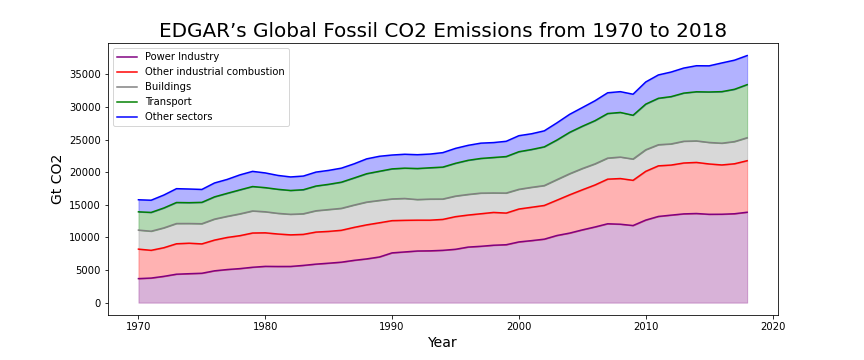
\includegraphics[width=5in]{edgars_co2_emissions.png}
\caption{Global Greenhouse Gas (GHG) emission per sector (see \cite{EDGAR19}). We see that the Power industry accounts for a large portion of global emissions, which provides insight as to where the largest opportunity for carbon reduction may be found.} 
\label{fig:edgars_co2_emissions}
\end{figure} 

Carbon offsetting is done via sequestration, which is the process where atmospheric carbon dioxide is captured and stored for the purpose of abating climate change. After carbon is captured, it goes mainly one of two ways: (a) permanently stored underground; or (b) converted into a carbon-containing product \cite{CBC19}. Currently, the market for corporate procurement for carbon removal is very undeveloped. However, there are a number of organizations that have made strides to address this issue; which include Amazon, Apple, BCG, Delta, Facebook, Google, Mars, Shopify, Stripe, Swiss Re, United and Velux \cite{Mic21}. Of the aforementioned, Shopify, Stripe and Microsoft are making carbon removal a core focus in their business. More specifically, Microsoft has a plan to remove carbon that they emit, and came to key conclusions. Namely, they can not meet current carbon negative commitments and estimate that they need to remove 6 Million tons of carbon in 2030. Hence, an RFP was sent out in 2020 and 79 applications were received and 15 organizations were selected representing 1.3 Million metric tons of carbon removal. Their project selection process was based on several criteria: (a) Global carbon removal potential; (b) Affordability targeting \$15 per MtCO$_{2}$; (c) climate equity; (d) technology innovation; and (e) other sustainability dimensions. 

In 2019, the National Academies of Sciences, Engineering, and Medicine investigated the likely market size for Negative Emissions Technologies (NET), where they discussed how much carbon uptake is needed to meet Paris Agreement goals \cite{NET19}. They estimate that $\sim$ 10 GtCO$_{2}$ / yr is required globally by midcentury and $\sim$ 20 GtCO$_{2}$ / yr globally by centuries end to meet these goals. Six key sequestration technologies are identified which are: (a) coastal carbon blue; (b) terrestrial carbon removal and sequestration; (c) bioenergy with carbon capture and sequestration (BECCS); (d) geological sequestration; (e) direct air capture;  and (f) carbon mineralization. Of these aforementioned technologies, the former four are ready for large-scale deployment; see Table \ref{table:net} for estimated potential rates across US and the Globe.

\begin{table}[h]
\centering
\begin{tabular}{ |c|c|c|c| } 
\hline
 Negative Emission Technology & Estimated Cost (\$/tCo$_{2}$) &\multicolumn{2}{ c |}{ Upper Bound for Safe Potential rate of CO$_{2}$ (GtCO$_{2}$/y)}  \\
  & & US & Global \\
\hline
Coastal blue carbon & L & 0.02 & 0.13  \\
Afforestation / Reforestation & L & 0.15 & 1  \\
Forest management & L & 0.1 & 1.5  \\
Agricultural soils & L to M & 0.25 & 3  \\
BECCS & M & 0.5 & 3.5-5.2  \\
Direct air capture & H & 0 & 0  \\
Carbon mineralization & M to H & unknown & unknown \\
Total &  & 1.02 & 9.13-10.83 \\
\hline
\end{tabular}
\caption{Estimated potential rates of CO$_{2}$ removal for various Negative Emission Technologies (measured in GtCO$_{2}$ / yr) for the US and across the globe (see \cite{NET19}), in terms of abundance, we see BECCS offers the best opportunity.}
\label{table:net}
\end{table}

\subsection{Problem Statement and Strategy}

We propose that token supply creation requires work, which include carbon sequestration followed by an auditing process working with various stakeholders involved in the process. The minting of new token supply can be compared to Bitcoin's Proof-of-Work (PoW) process popularly described as \emph{mining}, which is a completely automated and trustless process. However, the Carbon Renaissance (CR) token minting process will be governed by a regulatory work-flow process working through various stakeholders, which will be covered in this whitepaper. Many of the market dynamics that we know which drive price discovery via the Bitcoin miner network can be utilized to understand the market dynamics with this project. Such dynamics include: (a) geographical advantages characteristic to the local environment; (b) regulations particular to certain jurisdictions that allow for more cost effective sequestration; and (c) technological advancements.

The token supply can work in both an inflation/deflation environment depending on the system setup. Whereas other projects are either strictly deflationary or inflationary. For instance, we show via simulation that it is possible to have the supply reach a state of equilibrium where supply is constant.  This economic feature can make it attractive for large corporate organizations and governments to work with.

The CR process works in a cycle where the token can move to one of three different states over time (ie, statetokens). These states are: (a) Green; (b) Red; and (c) Black, each of which are usecase dependant. Green tokens (ie,  otherwise refereed to as base tokens) are purchased on exchanges and represent the potential of what can be utilized for carbon sequestration and are required to enter into the auditing process. Red tokens are non-tradable non-fungible tokens (NFT) and represent unique IOU contracts between stakeholders who have intentions to sequester carbon and those who offer the carbon sequestration service (see Fig. \ref{fig:red_to_green}). NFTs are unique digital assets that are stored on a blockchain and cannot be exchanged for one another, hence non-fungible. Some other example uses of NFTs are: (a) gaming; (b) digital art; (c) physical assets; and (d) digital collectibles.  Finally, Black tokens represent sequestered carbon. For instance, 100 Black tokens represent proof of 100 units of sequestered carbon and are created when Green tokens are burned. Black tokens are held privately and holding these tokens over time have the advantage of generating Green tokens which can generate additional revenue by being sold and recycled back into the system. We will be expounding further into the dynamics and utility behind these statetokens throughout this whitepaper.
 
\subsubsection{NFT Contracts}
\label{section:nft_tokens}

NFT contracts represent a legal framework and partnership with NFT issuances, see Fig. \ref{fig:red_green_issue} for the relationship between these stakeholders. They have the ability to white and black list those issuances to control the conversions, and have the authority to issue monetary redemptions of those NFT’s for when they break contract rules. Bundling these NFTs into these promissory contracts helps decouple concerns between pollution prevention companies and users of the credits. This idea allows stakeholders to seamlessly enable onboarding of partners without upfront costs. This disruptive technology allows for the seamless onboarding of partners without upfront costs and regulatory pressures that would otherwise slow down the workflow process using traditional means. We foresee that not requiring upfront investment and low barrier of entry for existing pollution prevention services will greatly increase the chance of network effects. Participants can target businesses by offering them the NFT and liquidity on the open market in exchange for their services. 

There is no responsiveness required on behalf of pollution prevention service providers as they can do as little or as much work as they want. Hence, no queues and no required customer acquisitions are required. All provided services are compensated (ie, provided they are audited and verified) and are motivated to be efficient by decoupling prevention of pollution from customer demand.

NFT tokens are minted upon the creation of each new contract, which is a promissory note to sequester a pre-determined amount of carbon. Once the obligation of the NFT contract is fulfilled, Green tokens are issued to the sequestration provider in exchange for service provided which in turn increases Green token supply. It should be noted that overall Green supply increases when NFTs are minted, but not tradable themselves until the contract is fulfilled. Hence, by definition total Green supply includes the aggregation of tradable Green tokens and non-tradable NFTs. Once fulfilled, these newly minted Green tokens are then bought by the pollution prevention company to meet their end of the contractual obligation laid out by the NFT. Pre-negotiated rates (even in non-token values if needed) are possible between stakeholders and CR for NFT-to-Green token exchange. This will give the ability to offload speculative concerns on the sequestration services part to CR. These speculative concerns can also be abated via raising capital to offer liquidity on the markets when needed as well.

\begin{figure}[h]
\centering
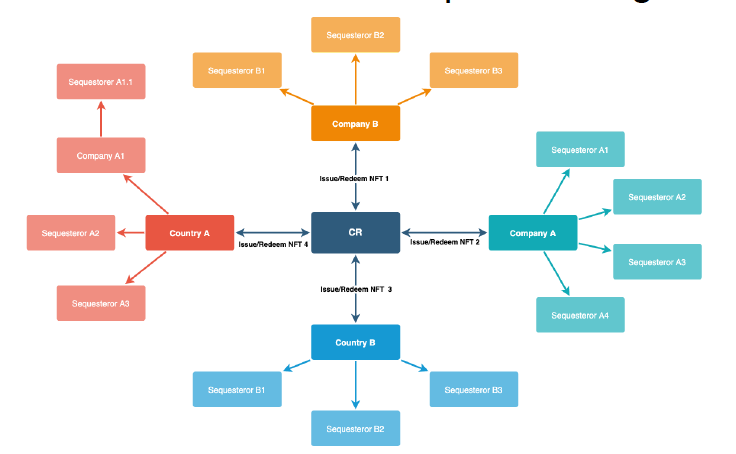
\includegraphics[width=4in]{red_green_issue.png}
\caption{Flow of NFT issuances and redemptions between pollution prevention stakeholders and sequesterors, which is all managed by CR and marks stakeholder relationship when burning Red tokens in exchange for Green} 
\label{fig:red_green_issue}
\end{figure} 

\subsection{Social Credit Component to UBI}

Using a carbon token incentive system would redistribute wealth, incentivize low carbon technology and avoid the environmental taxes which hit the world’s poor the hardest.

In some systems, the proposed UBI solutions are targeted to close the segregation between the rich and poor, but come at the cost of political interference. However these systems rarely work in practice because of the lobbying from the wealthy which have power to unilaterally dismiss such systems that intend to close the gap through taxation on rich and profitable corporations. Companies and people that move would ideally be met with similar taxation systems in other jurisdictions, however we foresee these other jurisdictions may or may not comply depending on their own policies and mandates to grow local economies through immigration of these wealthy people and companies.

Using the proposed carbon offset token program, governments can purchase carbon offsets, which can be considered as an efficient budget spending against environmental impacts of its economy and reduce taxes to those that inhibit environmentally responsible spending habits (such as buying local and not exceeding their carbon footprint quotas). Hence, creating a positive feedback loop to incentivize people to adapt their spending habits is a great way to find new efficiencies and invent \emph{greener} technologies due to increased demand for such technologies and services. The work here will be to assign carbon scores to goods and services and also assign spending against carbon ratings of goods and services. People that have a negative carbon footprint can be paid in Green tokens creating a powerful driver to reduce pollution and assigning monetary benefits which can be a social credit component to a UBI system, one which is tied to actual production and verified work.

\section{Proposed Design}

\subsection{Overview}

In the CR process, tokens move through a series of three states in an cyclic fashion. When the token is in a particular state, it can otherwise be defined as a statetoken, and (as discussed in the previous section) can take on the characteristics of one of three forms (ie, Green, Red, and Black). Upon initial issuance, 100M Green tokens are issued by CR, and over time this supply is set to decrease, while the supply of Red and Black tokens rise from zero to some steady-state equilibrium. Fig. \ref{fig:state_diagram} illustrates the state transition diagram where the nodes represent tokens and the arcs represent the direction and probability of a token transitioning to another over a unit of time.

Once the initial issuance of Green tokens has occurred, then pollution prevention stakeholders are issued one NFT asset for each partner, with assigned value based on their risk profile. The assigned value of the NFTs is denominated in Green tokens in the form of debt. This assigned value (denominated Green tokens) is based on the risk profile of the NFT holder (ie, akin to credit worthiness) which can be dynamically adjusted. These pollution prevention stakeholders can assign tokens to various sequesters competing in various markets for those contract NFTs. Those NFTs, which have a unique value based on jurisdiction or cost, are sent to these sequesters and audited based on circumstances with those issuers and partner stakeholders.

The NFT stays in the possession of the sequesterer until the work has been performed and verified via the auditing process (see Fig. \ref{fig:red_to_green}). Once complete, the NFT is burned and exchanged for Green tokens which is sold back to the pollution prevention company for revenue. Each NFT may have its own rules, regulations and even sequestering costs factoring in base asset to NFT cost ratios.

\begin{figure}[h]
\centering
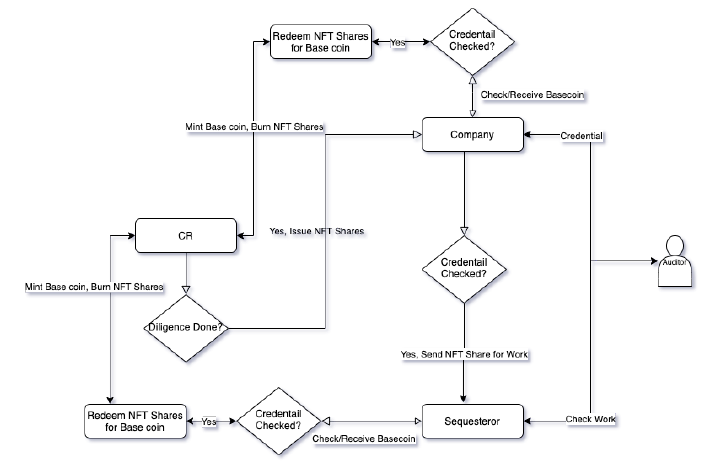
\includegraphics[width=4in]{red_to_green.png}
\caption{Process workflow illustrating how Green tokens are minted through the auditing of Red NFT contracts } 
\label{fig:red_to_green}
\end{figure} 

Burning Green tokens directly result in Black tokens directly by entering into the auditing process to apply credit to the pollution prevention stakeholder; see Fig. \ref{fig:green_to_black}. Once Green tokens are burned the holder will receive Black tokens. Holding these tokens is advantageous over extended periods of time, which will result in the minting of new Green tokens. For instance, if the state transition probability from Black to Green is 1\%, then 100 Black tokens will produce 1 Green token and 99 Black tokens when the state transitions across one monthly time unit.

\begin{figure}[h]
\centering
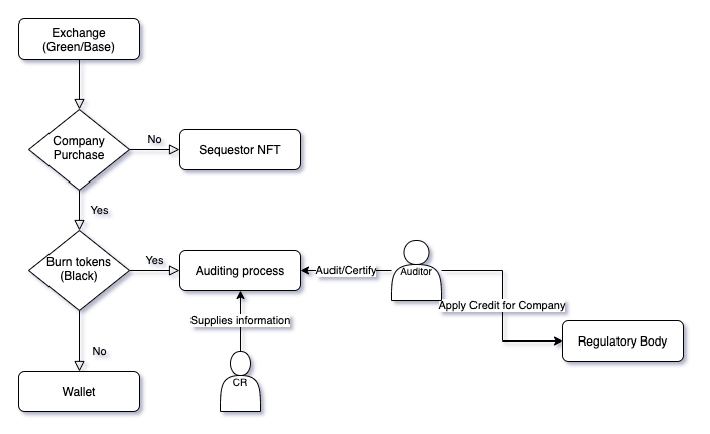
\includegraphics[width=4in]{green_to_black.png}
\caption{Process workflow illustrating how Green tokens are burned to mint Black tokens} 
\label{fig:green_to_black}
\end{figure} 

Green token supply increases as sequestering happens and decreases as companies accumulate and burn Green tokens as proof that they have credits. If the rate of sequestration exceeds the rate of credit consumed by companies, then the Green token supply is inflationary and is deflationary if sequestering does not adequately satisfy the burning of credits to black. For the deflationary case, sequestering services will naturally start to fill the demand and organically find equilibrium.

\subsection{Tokenized Company Shares}

It was requested that we create a fungible token for the purpose of share allocations in a company represented as a token product on blockchain. Also, these shares should not be transferable unless explicitly allowed by CR. We can enable this functionality on Syscoin through notary services which will allow a case-by-case basis for transaction authorization between peer-to-peer (P2P) transfers. Here are the following token specifications:

Token to sell to raise funds
\begin{itemize}
\item \textbf{Max supply}: 100M
\item \textbf{Precision}: 8
\item \textbf{Total raise}: sell 10M upfront @ \$34 US
\item \textbf{Token symbol}: GCX
\end{itemize}

Token to issue as NFT for companies
\begin{itemize}
\item \textbf{Max supply}: MAX
\item \textbf{Precision}: 8
\item \textbf{Token symbol}: CX
\end{itemize}

Token received from burning GCX or CX
\begin{itemize}
\item \textbf{Max supply}: MAX
\item \textbf{Precision}: 8
\item \textbf{Token symbol}: BCX
\end{itemize}

Individual NFT:
\begin{itemize}
\item \textbf{Precision}: 8
\item \textbf{Max supply}: MAX
\end{itemize}

\subsection{Supply Tokenomics}
\label{section:token_model}

Due to the nature of the supply dynamics involved with how each of the three tokens interact with each other, we have chosen to apply a Markov Chain simulation model to get a better understanding of what to expect under different conditions. For our problem, we setup the following transition matrix representing our business targets, where the frequency is monthly, and the states are represented as Green, NFT, and Burned respectively. To get an understanding of the underlying technicals, please refer to Appendix \ref{section:tokenomics}.

\begin{figure}[h]
\centering
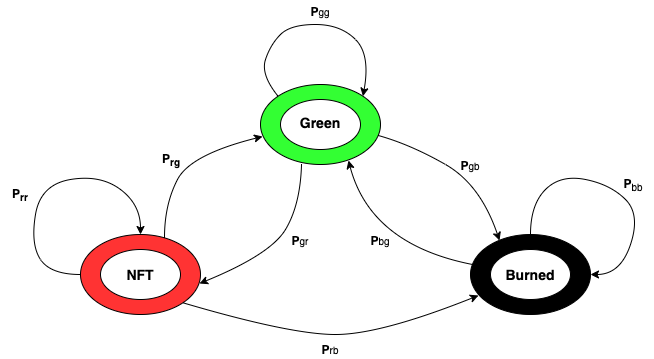
\includegraphics[width=4in]{state_diagram.png}
\caption{State transition diagram for Markov chain token model illustrating the probability of a token transitioning between states (ie, Green, NFT, and Burned) over a unit of time.} 
\label{fig:state_diagram}
\end{figure} 

\begin{table}[h!]
\centering
\begin{tabular}{|c c|c|c|c| } 
\hline
 & \multicolumn{4}{ c |}{ Next State } \\
 &  & Green & NFT & Burned \\
\hline
\multirow{ 3}{*}{Current State} & Green &  85\% & 0 & 15\% \\
& NFT & 33\% & 67\% & 0\\
& Burned & 1\% & 0 & 99\% \\
\hline
\end{tabular}
\caption{Transition state matrix for token model detailing probabilities of transitioning from current to next state over a monthly unit of time.}
\label{table:trans_state_matrix}
\end{table}

See Table \ref{table:trans_state_matrix} for the state transition matrix which represents our chosen business targets on how we believe the system will behave over time. For instance, for some stakeholder holding Green tokens, we are targeting 95\% of those tokens will remain in the hands of the holder at the next monthly time increment, and 5\% of those tokens will get burned into Black tokens. Since there is no current business case for a Green token to transition to a Red token, there is a 0\% chance that Green will transition to a Red token. With regards to NFTs, we are anticipating contract lengths to run 3 months on average. Hence, if a stakeholder runs back-to-back contracts over the course of a year, there is a 67\% chance that the holder will be holding their contract on any given month when they transition to the next month, and a 33\% chance that it will get burned. Finally, regarding Black tokens, since they represent proof of burn, we have decided to include an incentive for users that hold them, as a loyalty for users of the system so that they stay enticed to continue to stay engaged with the network. If a stakeholder is holding Black tokens, then 1\% of them will get converted back to Green at the next monthly time increment, which can then be reintegrated back into the cycle or sold back into the market. See Fig. \ref{fig:token_supply_sims} for simulation using methodology outlined in Appendix \ref{section:tokenomics} and Fig. \ref{fig:burned_minted} for simulated number of newly minted Green and Black tokens.

\begin{figure}
\centering
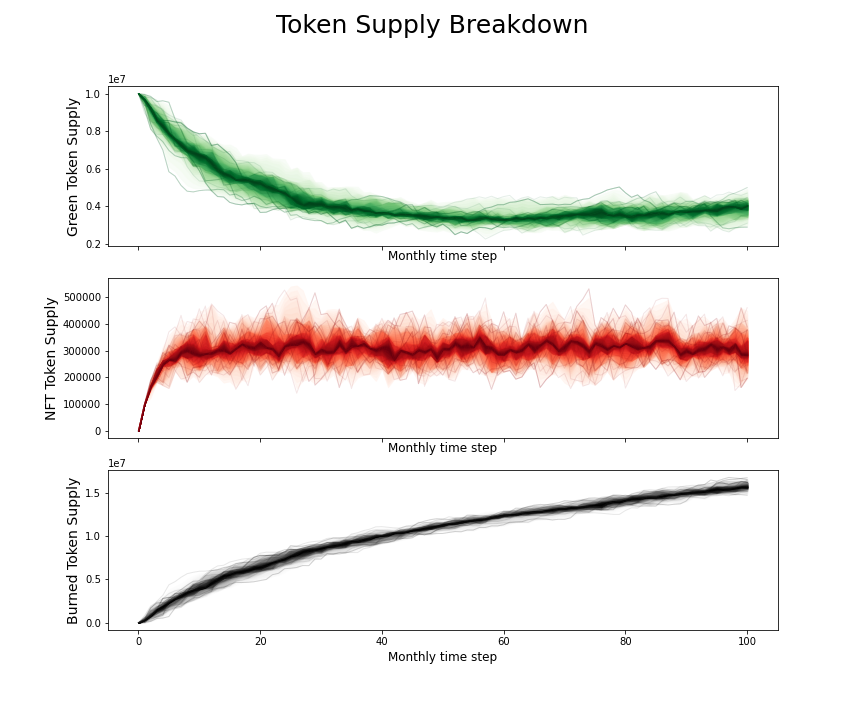
\includegraphics[width=4in]{token_supply_sims.png}
\caption{Markov Chain Token (MCT) model simulations assuming stationary transition probabilities applying the Beta distribution at each time point at a monthly frequency. The expectations of the transition probability matrix (\ref{e:transition_matrix}) was selected based on business targets. The simulation begins with 100M Green tokens, the bulk of which will transition to red and black tokens over time and eventually reach a state of equilibrium. When the system reaches steady-state, the expected supply of each of the Green tokens will become relatively stable with a slow increasing uptick over time.} 
\label{fig:token_supply_sims}
\end{figure} 

\begin{figure}
\centering
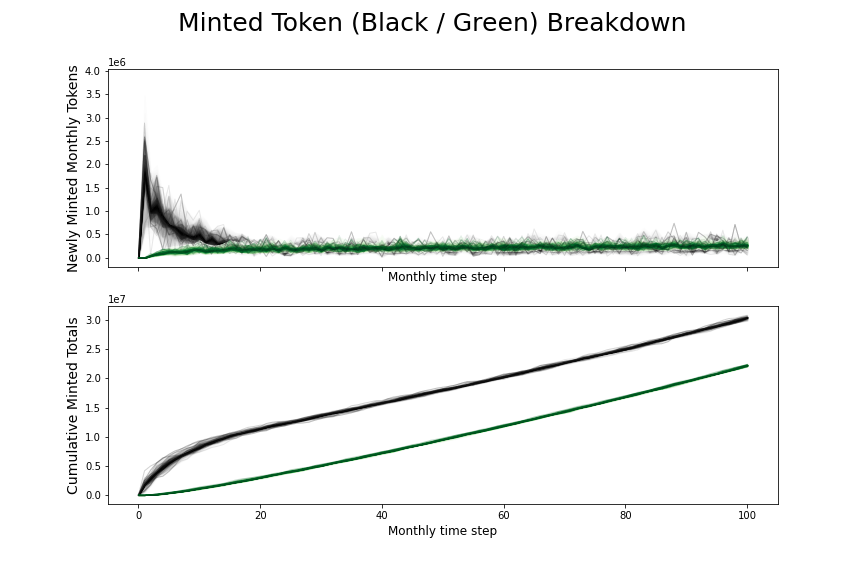
\includegraphics[width=4in]{burned_minted.png}
\caption{Newly minted green and burned tokens resulting from simulation model (\ref{e:token_supply_simulation}). Simulations of: (TOP) number of daily minted tokens; and (BOTTOM) cumulative number of daily minted tokens.} 
\label{fig:burned_minted}
\end{figure} 

\begin{figure}
\centering
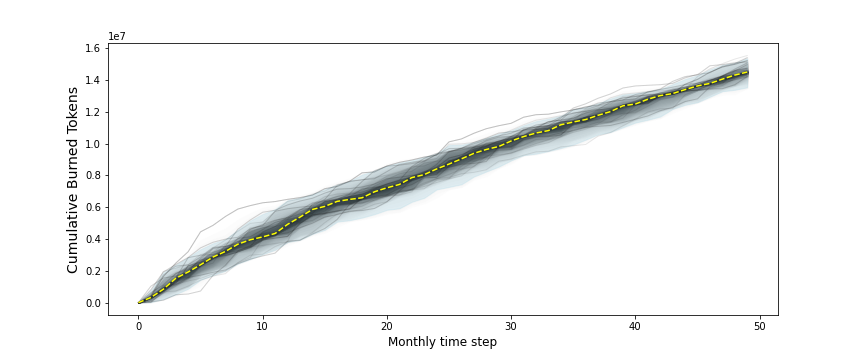
\includegraphics[width=4in]{burned_tokens.png}
\caption{Plot of simulated sequestered tons of carbon; this is determined by taking the cumulative sum of generated Black tokens overtime } 
\label{fig:burned_tokens}
\end{figure} 

\subsection{Revenue Model}

Both Green and Black tokens are fungible hence tradable on exchanges, but serve different ways to generate revenue. Green tokens are earned from sequestering carbon (ie, through NFT to Green token conversions) which can be sold for profit. Black tokens are earned through burning NFT or Green tokens. These Black tokens can be held privately which burn slowly over time (ie, at a predetermined rate set by CR) producing Green tokens that can be sold for profit or utilized back into the system. Aside from the tokens themselves, value added services such as software and wallets are other revenue generating options that companies may pay services for. 

Here, we approximate annual revenue (ie, first five years) based on simulated tonnes of sequestered carbon and estimated price of carbon; see Fig. \ref{fig:burned_tokens}. These estimated revenue figures are a back of the envelope calculation as we did not have any long term historical carbon price data. Thus, we use this as an exercise to get an idea of expected annual revenue generation. We use median carbon tax prices for 2021 as shown in Fig. \ref{figure:nation_carbon_taxes} as a proxy to the price of carbon. To determine the annual growth rate we applied the scheduled 2030 carbon tax price target of \$170 US from Canada's HEHE plan as a proxy. Considering that Canada's 2021 carbon tax price is $\sim$ \$32 US, that would work out to an annual growth rate of $\sim$ 20.5\%; see Table \ref{table:sim_revenue} for annual estimates and revenue projections.

\begin{table}[h]
\centering
\begin{tabular}{ |c|c|c|c|c|c| } 
\hline
 Year & median (tonnes) & lwr 5\% & upr 95\% & est. median price (USD)  & median revenue (USD)  \\
\hline
2023 & 9,056,000 & 8,470,000 & 9,789,000 & \$40.83 & \$369,792,000 \\
2024 & 12,315,000 & 11,959,000 & 12,619,000  & \$49.19 & \$605,749,000 \\
2025 & 14,963,000 & 14,443,000 & 15,448,000 & \$59.25 & \$865,887,000  \\
2026 & 17,620,000 & 17,284,000 & 17,836,000  & \$71.38 & \$1,257,642,000 \\
2027 & 20,293,000 & 19,994,000 & 20,690,000 & \$85.98 & \$1,744,829,000 \\
\hline
\end{tabular}
\caption{Simulated sequestered tons of carbon assuming transition matrix (see Table \ref{table:trans_state_matrix}) as business targets and corresponding median revenue. Since long-term historical market data is not available, we used Canada's current and future schedule 2030 carbon tax prices as a proxy to estimate annual growth rate \cite{Mck21}. Hence, we note that price estimates (ie, 5$^{th}$ column) are not based on rigorous mathematical analysis, but meant to provide an idea of revenue potential for strategic planning purposes.}
\label{table:sim_revenue}
\end{table}


\subsection{Implementation}

For the implementation of this project, we plan on utilizing Syscoin's Network Ethereum Virtual Machine (NEVM) as detailed in \cite{Sid21}. The NEVM consists of a four-layer tech stack that uses Bitcoin as the base layer, the EVM as the OS layer, Zero-knowledge Proof's (ZKP) as the SDK layer followed by an application layer. The motivation of a ZKP is to allow for one party (ie, prover) to convince another party (ie, verifier) of facts without revealing information (ie, zero knowledge), and is the gold standard for generalized computation scaling for blockchain applications. ZKPs enable one-time execution via a prover and enable aggregate proof checking instead of re-execution of complex transactions. The ZKP layer will be facilitated by a third-party software application called Starkware \cite{STA20} using a special type of ZKP called  Zero-Knowledge Scalable Transparent ARguments of Knowledge or zk-STARK \cite{Nas19}. It is estimated that this tech stack will be capable of delivering an upper bound of an approximated 210,000 transactions per second, see \cite{Sid21} for details.

Another reason for this choice of platform is Syscoin's capability of supporting NFTs, which are unique Syscoin-based digital assets that can not be replaced with something else. Some advantages of using Syscoin over other NFT platforms include divisibility and notary capabilities. Regarding divisibility, A good example of this is land ownership where fractions of such assets can be apportioned between multiple parties. Finally, developers will be able to employ Syscoin's notary capabilities by applying custom rule sets to transactions involving NFTs. This unique feature will allow for special rule sets required for the setting up of contracts between stakeholders.

\section{Project Management}

\subsection{Jurisdictional Dealings}

From time to time, companies may need cooperation with local governments who have requirements to fulfill quotas for its jurisdiction, which can be managed using a number of strategies. First, companies can buy directly from a local sequestration provider, and buy their NFT’s for a premium (ie, move to the front of the queue) which can been converted to Green tokens from CR (ie, pay requisite small fees for doing so). Upon fulfilling the needs of the NFT contract, tokens are then burned as described in Section \ref{section:nft_tokens}. Contracts would be directly created between NFT partners and sequestration companies, hence localized based on jurisdiction. Alternatively, companies can skip the auditing process and buy directly from CR via the aforementioned queue. Doing this puts more demand on those jurisdictions to produce more sequestration and would be an option if enough sequestration services are available. Finally, premiums paid for these higher demands are not factored into the Green token market unless larger market players drive prices upwards as global aggregate prices go up.

Evidence of the sequestration audit trail would need to be timestamped and recorded on the blockchain, which would be publicly accessible through a provided hyperlink in the asset public data field. This would be a live document that would update with signatures of auditors registered with Digital Identities and along with any associated metadata. The timestamped log will bring about transparency between consumed sequestrations, the actual registered audited sequestrations and allow one to audit that the supply of Green token accurately represents the audited sequestration amounts since one token can represent a certain amount of Carbon sequestration tonnage. It will allow companies to know what is available for consumption should there be requirements around jurisdictional consumption.

If companies require localized sequestration in exchange for burning Green tokens, then CR can select which sequestorers will qualify for which particular carbon credit application. Upon completion, tokens are burned and the time stamped audit trail is updated to reflect \emph{consumed} sequestrations. For instance, say MSFT requires 100 tons of US sequestration, and we have 100 tons of US sequestration in the audit trail, we can then choose those sequestrations and label them as consumed. Future US sequestration requests either need to pay the US sequestors, or wait for more sequestrations to register from US sequestors. However, under normal circumstances, the audit trail can be processed sequentially.

It would be ideal to manage such an effort at the global level (eg, under L'Accord de Paris) so that there are no jurisdictional requirements. Otherwise, the incentive would be to negotiate with companies directly. If the sequestration is fungible, the system can be more effectively managed through better supply stabilization and demand dynamics. For instance, this can be analogous to the Euro currency, where multiple countries, each with their own policies, utilize a single currency. This may be less ideal, but having this managed under a single policy may help avoid chances of corruption. However, we may not have control over this, and so we can employ this strategy upon further investigation, if need be.

\subsection{Competition}

There are a number of similar blockchain-based carbon crediting  projects that are currently underway globally. As far as tradable carbon credit tokens go, we have AirCarbon \cite{AirCarbon}, Carbonx \cite{Carbonx} and Verra. Each of these platforms focus on securitizing carbon credits with slight differences in how services will be delivered, like what we are proposing with CR. However, projects like SolarCoin \cite{SolarCoin} and Nori \cite{Nori} have more of a niche market. For instance, SolarCoin provides incentives to invest in solar installations which when monetized over time becomes effectively free.  Whereas the Verra program catalyses measurable climate action and sustainable development outcomes by enticing large-scale investment to activities to reduce emissions.

When it comes to securitizing carbon credits, CR is unique as it leverages the technological advantages that NFT provides so that pollution prevention companies and sequestration service providers can create contracts customized to the  stakeholders needs in accordance to the jurisdiction under which they fall.

\subsection{Cost of CO$_{2}$ Capture and Storage}

There have been a number of studies and whitepapers addressing methodological tools and surveys to help discover the cost of carbon sequestration \cite{Mck09,Gil18,Sch20,Dav00,Rub15,Rub07,Mck21}. To establish a global market for the cost of carbon would require some background understanding of the cost of CO$_{2}$, capture and storage (CCS) process. According to \cite{Rub15}, this can be sub-divided into two main purposes: (a) technology assessments to support things like capital investments and  technology selection; and (b) policy assessments to support things like legislative and regulatory issues. Methodologies into the determination of these carbon costs using a host of technical and economic assumptions as well as tabulated calculations have been well covered in \cite{Dav00,Rub07,Rub15}.

Marginal cost is a concept applied in economics that measures the cost of implementing additional units into a system. Whereas abatement cost is defined as the cost of reducing things that negatively impact the environment. Marginal abatement cost is the cost of reducing one unit of pollution, usually measured in metric tons of CO$_{2}$. A well-known tool for monitoring these costs is the marginal abatement cost curve, which is a widely used tool that was popularized by well-known organizations like Mckinsey through the utilization of their Greenhouse gas (GHG) abatement curve \cite{Mck09}. It is through the use of such tools that researchers and policy makers can collaborate to begin to take the first necessary steps of price discovery consolidated into a tradable global carbon market. 

Regarding actual costs, a research study for the northeastern and midwestern regions of the United States  suggests coal-sourced CO$_{2}$ emissions can be stored at a cost of \$52 to \$60 tonne, whereas the cost to store emission from natural-gas-fired plants ranges from approximately \$80 to \$90 \cite{Sch20}. A Harvard study has found fossil fuel power plants with carbon capture and storage costs estimated cost of \$43 to \$95 US per tonne \cite{Gil18}. In Canada, the current level of carbon tax is approximately \$30 per tonne (see Figure \ref{figure:nation_carbon_taxes}), and is anticipated to top out at \$50 per tonne in 2022. According to Canada's Healthy Environment and Healthy Economy (HEHE) plan, that figure is scheduled to rise to \$170 per tonne incrementally until the year 2030 \cite{Mck21}. We have a median global price of \~ \$28 per tonne by referring to available data on national carbon tax prices for 2021 from the World Bank in Fig. \ref{figure:nation_carbon_taxes}.

\begin{figure}[h]
\centering
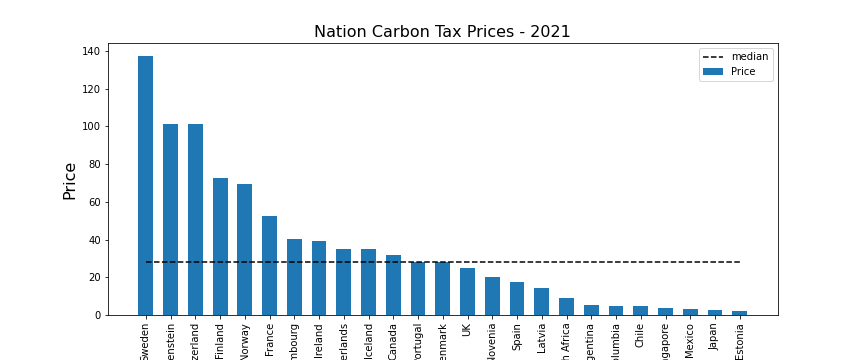
\includegraphics[width=5in]{nation_carbon_taxes.png}
\caption{National carbon tax prices for 2021; source can be found in \cite{WBank}. We see large variation between the various jurisdictions which provides insight as to which jurisdiction that may offer the best operating costs. This is akin to the variations in cost of electricity for various regions serving as the base cost for Bitcoin's PoW.} 
\label{figure:nation_carbon_taxes}
\end{figure} 

When trading the CR token on the market, we believe that market price governed by an aggregate of all CCS processes across all jurisdictions, namely the Average Sequestration Cost (ASC). We believe the market value of tradable CO$_{2}$ will be largely driven by this cost coupled with typical market speculation that is expected to fluctuate more drastically when this product is first introduced but will slowly temper over time.

\subsection{Carbon Exchange Rate: Speculative vs Stable}

Regarding the Green token to Carbon exchange rate, we conjecture that rate fluctuations will comprise of both a short term speculative component with an underlying rate discovery mechanism that will stabilize over time. This is done by allowing a floating speculative rate for companies requiring credits (ie, Green Tokens), while at the same time allowing for the setting of stable rates through the offloading of speculative risks for companies dealing with sequestering. Doing this allows for a better response to the supply side mechanics of Green tokens (ie, carbon credits).

Regarding the stable component we will work to keep the ratio as a constant 1:1; that is one Green token for one one ton of sequestered carbon. Doing this removes the need for governments and large enterprises having to make speculative purchases, hence making the system more usable. The number of new minted tokens depends on the number of new tons of carbon that are being introduced into the atmosphere. If the amount of new carbon being sequestered globally is greater than new pollution, then Green tokens become deflationary, otherwise it's inflationary.

Alternatively, regarding the speculative component, we begin the process with a 1:1 ratio, however the ratio changes as tokens are burned over time. Hence, making one ton of carbon to be less than one Green token. This model adds speculation enticing enterprises to purchase and remove tokens from the supply which reduce costs over time and also for potential gains. While the dollar's cost value remains consistent, the number of tokens required for one ton of carbon emissions drops, hence putting deflationary pressures on the supply.

\subsection{Markets}

From the standpoint of corporations interested in pollution prevention, there are currently a decent number of initiatives coming from the tech sector. Hence, due to the tech related nature of this project, we believe many of our first customers will come from this sector due to their appetite for innovation in disruptive technologies like blockchain. Such companies that have already made mandates in this sector include: Microsoft, Amazon, Apple, Facebook, Google, Mars, Shopify and Stripe \cite{Mic21}. Also, we feel that there may be opportunities in the blockchain space itself offsetting carbon expended for PoW based projects. In the event of enforced regulation, we foresee that there will be willpower  to develop this particular market. 

As per Fig. \ref{fig:edgars_co2_emissions}, the next obvious choice would be the power industry  \cite{Sch20,Gil18} as it represents the highest portion of carbon emissions by major sector. Given the fact that the cost of offsetting for fossil fuel plants range from \$43 to \$95 US per tonne \cite{Gil18}, it makes sense for this industry to outsource this offsetting to sequestration providers for a cheaper cost. Hence, providing another opportunity in the new carbon market.

\subsection{Limitations}

The PoW process in Bitcoin is a trustless system as its all managed by code. However, the work for new token minting is created by fulfilling audits resulting from carbon sequestration. Hence, the carbon sequestration auditing process is subjective and not trust-less as it can be compromised by bad actors. Hence, concessions will be put in place to thwart such potential activity.

\section{Summary}

Global greenhouse gas emissions have been climbing consistently over the past 50 years which has given rise to climate change. Within these emissions, the power industry sector represents the largest contribution. Also, bioenergy with carbon capture and sequestration represents the technology with the most promise. If we consider using carbon tax prices as a proxy, countries like Chile, Columbia, Mexico, Estonia and Argentina represent cost effective jurisdictions for sequestration. According to our research carbon sequestration projects exhibiting some or all of the features represent the best opportunities.

There are several new companies working to bring new carbon sequestration mechanisms to market. Living Carbon uses genetic engineering to improve how trees break down a toxic byproduct of photosynthesis which results in photosynthesis-enhanced trees that grow 30-54\% faster \cite{LC21}. Svante Inc. is a Silicon Valley based startup that helps capture carbon from industrial cement, steel, and other manufacturing plants which has just raised \$ 25M CND in capital from the Canadian government \cite{SA21}. Holy Grail is a Silicon Valley based startup that has developed a device that cost effectively separates CO$_{2}$ from the air and has raised \$2.7M US in seed capital \cite{HG21}.

Given the fact that there is no open market for carbon sequestration we propose a carbon offset design program using blockchain tokenization for our design. The advantages to using such technology are: (a) minimizes red tape allowing for improved accessibility; (b) improves efficiency by allowing for direct peer-to-peer transactions eliminating third party involvement; (c) provides transparency and trust on an immutable public ledger database; (d) provides global access across various jurisdictions; and (e) drives new payment innovations that go beyond the limitations of current fiat money system. Our proposal consists of three tokens (Green, Red, and Black tokens); the action of transitioning from one token state to another is called burning. Green tokens are required to enter into the carbon offsetting process directly and are awarded as work done via the auditing process. Next, NFT tokens serve as IOU contracts to sequester carbon. Finally, Black tokens serve as proof of burn which can be staked to gain more Green tokens as an incentive for users to retain engagement with the network. We are targeting that 10\% of Green token supply and 33\% of NFTs will get burned every month which we estimate will generate nearly \$900M US in annual revenue by 2025.

\section{Appendix}

\subsection{Tokenomics}
\label{section:tokenomics}

Assume we are given the following stochastic (Markov) matrix:

\begin{equation}
P_{\mu}  = 
\begin{bmatrix}
p_{g,g} & p_{g,r}  & p_{g,b} \\
p_{r,g} & p_{r,r}  & p_{r,b} \\
p_{b,g} & p_{b,r} & p_{b,b} 
\end{bmatrix}
\label{e:transition_matrix}
\end{equation}

where each element is non-negative and each row sums to one. Each row of the $m \times n$ matrix $P_{\mu}$ can be regarded as a probability mass function over $n$ possible outcomes. For instance, element $p_{g,b}$ represents the probability of a green token transitioning to a black token between states. In Fig \ref{fig:state_diagram}, we represent this Markov process as a directed graph with edges labelled by the transition probabilities in (\ref{e:transition_matrix}).

Let's assume $\{X_{t}\}$ is a Markov chain with stochastic matrix $P_{\mu}$, and the distribution of $X_{t}$ to be $\psi_{t}$. Hence, if we let the initial distribution of $\psi_{0} = [1,0,0]$, the probability distribution of $X_{t}$ can be determined via:

\begin{equation}
X_{t} \sim \psi_{0}P^{t}
\label{e:pow_vs_pos}
\end{equation}

Hence, the estimated token supply at time $t$ is given by:
\begin{equation}
\hat{S}_{t} = (S_{0} + \alpha N_{t})\psi_{0}P^{t}
\label{e:token_supply}
\end{equation}
where $S_{0}$ is the initial token supply (ie, 100M Green, 0 NFT and 0 Black tokens), $N_{t}$ represents the NFT IOU rate, and $\alpha \in [0,1)$ represents the global quality factor (eg, 0.9).

\subsubsection{Token Model Simulation}

To simulate transition probabilities in $\mathbf{P}_{t}$, we use the Beta distribution:
\begin{equation}
\mathbf{p}_{m,n,t} \sim Beta(\alpha_{m,n},\beta_{m,n})
\end{equation}
where $m$ is the current state, $n$ is the previous state and $\beta_{m,n} = 1-\alpha_{m,n}$. The parameters $\alpha_{m,n}$ and $\beta_{m,n}$ are selected such that $E\{\mathbf{P}_{t}\}$ = $P_{\mu}$. It is important to keep in mind that this is a stationary model, hence the expected values are invariant to time. We ensure that the rows of the simulations of $\mathbf{P}_{t}$ sum to one by applying the following normalization:
\begin{equation}
p_{m,n,t}'= \dfrac{p_{m,n,t} }{  \sum_{n} p_{m,n,t}  }.
\end{equation}
where $p_{m,n,t}$ represents an element of $\mathbf{P}_{t}$ at time $t$. The simulated token supply  at time $t$ is defined as:
\begin{equation}
\hat{\mathbf{S}}_{t} =(S_{0} + \alpha N_{t})\psi_{0}\mathbf{P}_{t}^{t}
\label{e:token_supply_simulation}
\end{equation}

\subsubsection{Limitations}

Regarding limitations, this model assumes that transition probabilities in (\ref{e:transition_matrix}) are stationary over time. Since we do not have data, we make this simplified assumption for the sake of making simulated projections based on expected targets. Once data has been obtained, the next step would be to investigate non-stationary structure in the transition probabilities over time. These non-stationary structures would be modelled and factored into the existing model, which will allow for the upgrade from a planning tool into an actual predictive model.

\label{section:summary}

\begin{thebibliography}{1}

\bibitem{Kal96} E. Kalnay et. al., \textit{The NCEP/NCAR 40-Year Reanalysis Project}, Bulletin of the American Meteorological Society, 1996, pp. 77437-471

\bibitem{Ten00} J.B. Tenenbaum, V. Silva and J.C. Langford, \textit{A Global Geometric Framework for Nonlinear Dimensionality. Reduction}. Science, Vol. 290, No. 5500, 2000.

\bibitem{Hij05} R.J. Hijmans, S.E. Cameron, J.L. Parra, P.G. Jones and A. Jarvis, \textit{Very High Resolution Interpolated Climate Surfaces for Global Land Areas}, International Journal of Climatology, Vol. 25, 2005.

\bibitem{Glo21} \textit{Global Warming of 1.5 ºC}, Accessed on: Jul 2021. [Online]. https://www.ipcc.ch/sr15/

\bibitem{EDGAR19} \textit{European Commission, Joint Research Centre (EC-JRC)/Netherlands Environmental Assessment Agency (PBL)}. Emissions Database for Global Atmospheric Research (EDGAR), release EDGAR v5.0 (1970 - 2015), Nov 2019.

\bibitem{Liu20} Z. Liu et al.,  \textit{Global energy review: CO2 emissions in 2020}, Dec 2021. Accessed on: Dec 2020 [Online]. Available: https://arxiv.org/abs/2012.00854

\bibitem{CBC19} E. Chung, \textit{Carbon capture: What you need to know about catching CO2 to fight climate change}, CBC Science, Sep 2019, Accessed on: Jul 2021. [Online]. https://www.cbc.ca/news/science/carbon-capture-faq-1.5250140

\bibitem{Mic21}  \textit{Microsoft carbon removal: Lessons from an early corporate purchase}, Accessed on: Jul 2021. [Online]. https://www.microsoft.com/en-us/corporate-responsibility/sustainability/carbon-removal-program

\bibitem{NET19} National Academies of Sciences, Engineering, and Medicine, \textit{Negative Emissions Technologies and Reliable Sequestration: A Research Agenda (2019)}, The National Academies Press, Washington, DC, 2019. 

\bibitem{AirCarbon} \textit{A digital exchange focused on eliminating market friction in a carbon constrained economy.}, Accessed on: Jul 2021. [Online]. https://www.aircarbon.co/

\bibitem{Sid21} J. Sidhu, \textit{A Design For An Efficient Coordinated Financial Computing Platform}, Feb. 2021, Accessed on: Jul 2021. [Online]. https://jsidhu.medium.com/a-design-for-an-efficient-coordinated-financial-computing-platform-ab27e8a825a0

\bibitem{STA20} Starkware Team, Rescue STARK Documentation — Version 1.0, Jul 2020

\bibitem{Nas19} L.T. do Nascimento, S. Kumari, and V. Ganesan, Zero Knowledge Proofs Applied to Auctions, May 2019, Accessed on: Feb 2021 [Online]. Available: https://courses.csail.mit.edu/6.857/2019/project/18-doNascimento-Kumari-Ganesan.pdf

\bibitem{Carbonx} \textit{A Personal Carbon Trading Inc.}, Accessed on: Jul 2021. [Online]. hhttps://www.carbonx.ca/

\bibitem{SolarCoin} \textit{SolarCoin is a cryptocurrency that incentivizes a solar-powered planet}, Accessed on: Jul 2021. [Online]. https://solarcoin.org/

\bibitem{Nori} \textit{The Nori Carbon Removal Marketplace}, Accessed on: Jul 2021. [Online]. https://nori.com/

\bibitem{Mck09} McKinsey \& Company, \textit{Impact of the Financial Crisis on Carbon Economics: Version 2.1 of the Global Greenhouse Gas Abatement Cost Curve}, 2009. 

\bibitem{Gil18} K. Gillingham and J. H. Stock \textit{The Cost of Reducing Greenhouse Gas Emissions} Journal of Economic Perspectives, Vol. 32, No. 4, Fall 2018, pp. 53–72

\bibitem{Sch20} W. Schmelz, G. Hochman, K. Miller, \textit{Total cost of carbon capture and storage implemented at a regional scale: northeastern and midwestern United States}, Interface Focus, 10 (5), 2020, pp. 20190065.

\bibitem{Dav00} J. David, H.J. Herzog, \textit{The cost of carbon capture}, Fifth International Conference on Greenhouse Gas Control Technologies (GHGT-5), Cairns, Australia, Aug 13–16, 2000.

\bibitem{Rub15} E. Rubin, J. David and  H.J. Herzog, \textit{The cost of CO2 capture and storage}, International Journal of Greenhouse Gas Control, Vol. 40, Sept. 2015, pp. 378-400

\bibitem{Rub07} E. Rubin, C. Chen and A. Rao, \textit{Cost and performance of fossil fuel power plants with CO2 capture and storage}, Energy Policy, Vol. 35, Issue 9, Sept. 2007, Pages 4444-54

\bibitem{Mck21} R. McKitrick and E. Aliakbari, Estimated Impacts of a \$170 Carbon Tax in Canada, Fraser Institute, 2021

\bibitem{WBank} \textit{Worldbank Carbon Pricing Dashboard}, Accessed on: Jul 2021. [Online]. https://carbonpricingdashboard.worldbank.org/map\_data

\bibitem{Microsoft21} \textit{Microsoft Bought Carbon Credits Through Cosmos Blockchain}, Accessed on: Jul 2021. [Online]. https://thecoinshark.net/blockchain-news/microsoft-bought-carbon-credits-through-cosmos-blockchain

\bibitem{DOE16} \textit{Carbon Capture, Utilization, and Storage: Climate Change, Economic Competitiveness, and Energy Security}, US Department of Energy, 2016, Accessed on: Jul 2021. [Online]. https://www.energy.gov/fe/downloads/doe-white-paper-carbon-capture-utilization-and-storage

\bibitem{Cri20} M. Crippa, D. Guizzardi, M. Muntean, and E. Schaaf, \textit{Fossil CO2 emissions of all world countries - 2020 Report}, Publications Office of the European Union, Luxembourg, Sept 2020.

\bibitem{CDCS05} \textit{Carbon Dioxide Capture and Storage}, Intergovernmental Panel on Climate Change, Cambridge University Press, 2005.

\bibitem{LC21} \textit{Living Carbon: Engineering faster-growing, more durable trees}, Accessed on: Aug 2021. [Online]. https://lowercarboncapital.com/company/livingcarbon/


\bibitem{SA21} \textit{Ottawa invests \$25 million in B.C.-based startup to help build 'Silicon Valley of carbon capture industry' }, Jul 2021, Accessed on: Aug 2021. [Online]. https://financialpost.com/commodities/energy/oil-gas/ottawa-invests-25-million-in-b-c-based-carbon-capture-startup

\bibitem{HG21} \textit{Holy Grail}, Accessed on: Aug 2021. [Online]. https://www.holygrail.ai/

\end{thebibliography}



\end{document}